\documentclass[11pt]{article}
%%%% Load Packages %%%%
\usepackage[utf8]{inputenc}
\usepackage[english]{babel}
\usepackage{indentfirst}
\usepackage{color}
% \usepackage{url}
\usepackage{hyperref}
\usepackage[citestyle=authoryear, bibstyle=authoryear, sorting=nyt]{biblatex}
\usepackage{caption}
% \usepackage{etoolbox}
\usepackage{fancyhdr}
\usepackage{geometry} %[margin=1in]
%\usepackage[absolute]{textpos}
\geometry{
	top=1in, % Top margin
	bottom=1in, % Bottom margin
	left=1in, % Left margin
	right=1in, % Right margin
%	showframe, % Uncomment to show how the type block is set on the page
}
\usepackage{pdflscape}
\usepackage{graphicx}
\usepackage{parskip}
\usepackage{setspace}
\usepackage{titlesec}
\usepackage{titletoc}
\usepackage{booktabs}
\usepackage{multirow}
%\usepackage{endnotes} % Use end notes instead of footnotes
%\let\footnote=\endnote % Use end notes instead of footnotes

% Adjust marginparwidth before loading todonotes/changes
\setlength{\marginparwidth}{2cm}
\usepackage{changes} % Use [final] to accept all changes; remove [final] to track changes
% Define author for suggestions
\definechangesauthor[name={Matt Carson}, color=red]{MC}

\usepackage[autostyle, english = american]{csquotes}
\MakeOuterQuote{"}
\usepackage[acronym, nogroupskip]{glossaries}
\makeglossaries

%\titleformat{\section}{\fontsize{12}{14}\bfseries\centering}{\thesection}{0.5em}{}

%%%% Include acronyms file %%%%
%%%% List of Acronyms and abbreviations %%%%

\newacronym{afl}{AFL}{American Federation of Labor}
\newacronym{aflcio}{AFL-CIO}{American Federation of Labor-Congress of Industrial Organizations}
\newacronym{anga}{ANGA}{America's Natural Gas Alliance}
\newacronym{btc}{BTC}{Building Trades Council}
\newacronym{cba}{CBA}{Collective Bargaining Agreement}
\newacronym{cio}{CIO}{Congress of Industrial Organizations}
\newacronym{csb}{CSB}{U.S. Chemical Safety and Hazard Investigation Board}
\newacronym[
    description={Community Workforce Agreement (also called Project Labor Agreement [PLA])}
]{cwa}{CWA}{Community Workforce Agreement}
\newacronym{dapl}{DAPL}{Dakota Access Pipeline}
\newacronym{efca}{EFCA}{Employee Free Choice Act}
\newacronym{iam}{IAM}{International Association of Machinists and Aerospace Workers}
\newacronym{ibew}{IBEW}{International Brotherhood of Electrical Workers}
\newacronym{ilgwu}{ILGWU}{International Ladies Garment Workers Union}
\newacronym{ilwu}{ILWU}{International Longshore and Warehouse Union}
\newacronym{iupat}{IUPAT}{International Union of Painters and Allied Trades}
\newacronym{iww}{IWW}{Industrial Workers of the World}
\newacronym{jatc}{JATC}{Joint Apprenticeship Training Committee}
\newacronym{lcca}{LCCA}{Labor Coalition for Community Action}
\newacronym{lcsp}{LCSP}{Labor Campaign for Single Payer}
\newacronym{liuna}{LIUNA}{Laborers' International Union of North America}
\newacronym{lmrda}{LMRDA}{Landrum-Griffin Labor-Management Reporting and Disclosure Act}
\newacronym{nabtu}{NABTU}{North America's Building Trades Unions}
\newacronym{nepa}{NEPA}{National Environmental Policy Act}
\newacronym{nlra}{NLRA}{National Labor Relations Act}
\newacronym{nlrb}{NLRB}{National Labor Relations Board}
\newacronym{ocaw}{OCAW}{Oil, Chemical and Atomic Workers Union}
\newacronym{opcima}{OPCIMA}{Operative Plasterers' and Cement Masons' International Association}
\newacronym{oshact}{OSH Act}{Occupational Safety and Health Act}
\newacronym{owiu}{OWIU}{Oil Workers International Union}
\newacronym{pace}{PACE}{Paper, Allied-Industrial, Chemical, and Energy Workers International Union}
\newacronym[
    description={Project Labor Agreement (also called Community Workforce Agreement [CWA])}
]{pla}{PLA}{Project Labor Agreement}
\newacronym{proact}{PRO Act}{Protecting the Right to Organize Act}
\newacronym{rwdsu}{RWDSU}{Retail, Wholesale, and Department Store Union}
\newacronym{seiu}{SEIU}{Service Employees International Union}
\newacronym[
	description={United Association of Journeymen and Apprentices of the Plumbing and Pipe Fitting Industry}]
	{ua}{UA}{United Association of Plumbers and Pipefitters}
\newacronym{uaw}{UAW}{United Auto Workers}
\newacronym{ufcw}{UFCW}{United Food and Commercial Workers}
\newacronym{ugccwa}{UGCCWA}{United Gas, Coke, and Chemical Workers of America}
\newacronym{umwa}{UMWA}{United Mine Workers of America}
\newacronym{upiu}{UPIU}{United Paperworkers' International Union}
\newacronym[
	description={United Steel, Paper and Forestry, Rubber, Manufacturing, Energy, Allied Industrial and Service Workers International Union}
]{usw}{USW}{United Steelworkers}

%%%% Head height %%%%
\setlength{\headheight}{15pt}

%%%% Line spacing %%%%
\setstretch{2}

%%%% Paragraph spacing %%%%
\setlength{\parskip}{0pt}

%%%% Define indentation length %%%%
\newlength{\myindent}
\setlength{\myindent}{0.5in}

%%%% Set the hanging indent %%%%
\setlength{\bibhang}{\myindent}

\AtEveryBibitem{
	\clearfield{issn}
	\ifentrytype{book}{\clearfield{isbn}}{}
    \clearfield{urlyear}
    \clearfield{urlmonth}
    \clearfield{urlday}
}

%%%% Redefine the citation command to use a colon instead of a comma and pp. %%%%
\DeclareFieldFormat{postnote}{#1}
\DeclareFieldFormat{multipostnote}{#1}

% Redefine the URL format to not use \texttt style
%\DeclareFieldFormat{url}{\href{#1}{#1}} % This will format the URL in the regular text font

% Optionally, redefine the DOI and eprint formats similarly if you use them
%\DeclareFieldFormat{doi}{\href{https://doi.org/#1}{#1}}
%\DeclareFieldFormat{eprint}{\href{https://arxiv.org/abs/#1}{#1}}

%%%% Use colon (ASA Style) in-text citations (author year: page) %%%%
\renewcommand*{\postnotedelim}{\addcolon}

%%%% Set global text alignment to ragged-right %%%%
%\raggedright

%%%% Paragraph indentation %%%%
\setlength{\parindent}{\myindent}

%%%% Font %%%%
% \setmainfont{Times New Roman}

%%%% Define variables for reused text or dimensions %%%%
% Full title
\newcommand{\fullTitle}{Construction Union Agreements:\par{}Union Organizing in Historical-Comparative Perspective}
% Short title
\newcommand{\shortTitle}{CONSTRUCTION UNION AGREEMENTS}

% Standardize image width
\newcommand{\imageWidth}{0.8\textwidth}

%%%% Page style %%%%
\pagestyle{fancy}
\fancyhf{} % clear all header and footer fields
%\fancyhead[R]{\thepage} % page number on the right side
\fancyhead[R]{\hyperlink{toc}{\thepage}} % page number on the right side, linked to the TOC
\fancyhead[L]{\small \shortTitle}
\renewcommand{\headrulewidth}{1pt} % header rule

% Customize abstract page
\renewenvironment{abstract}
  {\par\noindent\centering\textbf{\fullTitle}\par}
  {\noindent\raggedright}
%  {\par}

% Redefine the quote environment
\renewenvironment{quote}
  {\list{}{\leftmargin=\parindent\rightmargin=0pt}%
   \item\relax}
  {\endlist}
  
% Redefine the quote environment to make it single-spaced 
% and remove vertical space before and add one at the end
\AtBeginEnvironment{quote}{\singlespacing\setlength{\topsep}{0pt}\setlength{\partopsep}{0pt}}
\AtEndEnvironment{quote}{\vspace{0.5\baselineskip}}

% Custom command \acrparen to place acronyms in parentheses
% \acrparen
\newcommand{\acrparen}[1]{(\acrshort{#1})}

% Custom command to reference section number and name
% \fullref
\addto\extrasenglish{\def\sectionautorefname{Section}}
\addto\extrasenglish{\def\subsectionautorefname{Section}}
\addto\extrasenglish{\def\subsubsectionautorefname{Section}}
\newcommand{\fullref}[1]{\autoref{#1}: ``\nameref{#1}"}

% Command to use \textcite in the possessive form
\newcommand{\poscite}[1]{\citeauthor{#1}'s (\citeyear{#1})}
%	%%%%%%%%%%%%%%%
%			Document Begins         %
%			Preliminary Pages 		  %
%	%%%%%%%%%%%%%%%
\addbibresource{1_SOC_Honors.bib}
%%%% Title Page %%%%
\begin{document}
\setstretch{1.25} % Set line spacing
\begin{titlepage}
  \thispagestyle{fancy}
  \pagenumbering{gobble} % Turn off page numbering for the title page
  \fancyhead[L]{Running Head: \shortTitle}
  \renewcommand{\headrulewidth}{0pt} % header rule
  {\centering
  \vspace*{2in}
  \fullTitle*\par
  \vspace{1.2in}
  {Matthew A. Carson\par}
  \vspace{12pt}
  Department of Sociology\par
  University of California, Los Angeles\par
  \vspace{0.5in}
  {June 8, 2024\par}}
 \vfill
 \noindent{}*This is an abbreviated version of the author's sociology departmental honors thesis. For the sake of brevity, some analyses have been excluded. The entire, unabridged thesis is available at https://bit.ly/SocThesis
\end{titlepage}

% Blank page so that the abstract does not begin on the back of the cover page.
% Blank page
\thispagestyle{empty} % Remove header and footer

\vspace*{\fill}
\hspace*{\fill}
\begin{center}
    \noindent{}\textit{This page intentionally left blank}
\end{center}
\hspace*{\fill}
\vspace*{\fill}

\clearpage

% Set page numbering to Roman for preliminary pages
\pagenumbering{roman}
\setstretch{2}
%\titlespacing*{\abstract}{0pt}{0pt}{0pt}

% Add abstract page
\begin{abstract}
US Building Trade unions organize their workers differently. Most labor unions compel employers to negotiate, but the Building Trades engage in voluntary negotiations, relying on workers' skill levels rather than strike leverage. This approach correlates with their frequent political deviations from the broader US labor movement, particularly in opposing progressive environmental policies, aligning more closely with the petrochemical industry on environmental issues, and not supporting single-payer healthcare. One view is that unions pursue their members’ interests narrowly, sacrificing broader working-class interests if they feel it is necessary to secure work for their members, and some suggest that the conservative stance of the Building Trades stems from their craft union tradition, in which workers are organized by craft and skill instead of by industry. However, using historical-comparative methods, I show that these arguments do not hold. Petrochemical unions have supported progressive policies, and other craft-based unions have endorsed single-payer healthcare. However, unlike the Building Trades, those unions have never used voluntary agreements. Consequently, they have experienced more conflicts with employers. These findings challenge traditional views and suggest that the Building Trades' conservative negotiation strategies significantly shape their political and policy positions and reinforce an employer-union dynamic that limits challenging management.
\end{abstract}

\clearpage

% Add table of contents (TOC)
\setstretch{1.25}
\hypertarget{toc}{}
\tableofcontents
\clearpage

% List of Figures
\listoffigures

% List of tables
\listoftables

\clearpage


%	%%%%%%%%%%%%%%%%%%%	%
% Define custom section headings			%
%	%%%%%%%%%%%%%%%%%%%	%
%%%% Parts %%%%
\titleformat{\part}[block]
	{\normalfont\Large\bfseries}
	{\thepart.}
	{6pt}
	{\Large\MakeUppercase}

%%%% Sections %%%%%
\titleformat{\section}[block]
	{\normalfont\fontsize{12}{14}\selectfont\bfseries}
	{\thesection.}
	{0.25em}
	{}

%%%% Subsections %%%%
\titleformat{\subsection}[block]
	{\itshape\bfseries}
	{} % \thesubsection.
	{0pt} % 0.25em
	{}

%%%% Subsubsections %%%%
\titleformat{\subsubsection}[runin]
	{\normalfont\itshape\bfseries}
	{\hspace{\myindent}} % \thesubsubsection.
	{0pt} % 0.25em
	{}[.]%{\hspace{0em}}%[\hspace{2pt}]

%%%% Paragraphs %%%%
\titleformat{\paragraph}[runin]
	{\normalfont\itshape\bfseries} % Normal font, italic, bold
	{} % \hspace{\myindent}\theparagraph. % Label (you can add numbering here if needed)
	{0.25em} % Separation between the label and the title
	{} % Additional formatting
	[.]

% Adjust spacing before and after sectioning commands
\titlespacing*{\part}{0pt}{0pt}{10pt}
\titlespacing*{\section}{0pt}{0pt}{0pt} % \baselineskip
\titlespacing*{\subsection}{0pt}{0pt}{0pt}
\titlespacing*{\subsubsection}{0pt}{0pt}{0.5em}
\titlespacing*{\paragraph}
  {\myindent} % Left margin (you can set this to \parindent to align with paragraph indentation)
  {0pt} % Space before the paragraph title
  {0.5em} % Space after the paragraph title

% \titlecontents{subsubsection}
  % [5em]                       % 1. Indentation
  % {}                          % 2. Above code
  % {}                          % 3. Numbered entry format
  % {}                          % 4. Formatting of numbered entry
  % {\hspace{0.25em}\titlerule*[0.75em]{.}\contentspage}       % 5. Page number format
  % []                          % 6. Below code


%%%%%%%%%%%%%%%%%%%%%%%
%%					Main document starts			  %%
%%%%%%%%%%%%%%%%%%%%%%%
% Set to double-spacing
\setstretch{2}

\clearpage
%% Blank page
\thispagestyle{empty} % Remove header and footer

\vspace*{\fill}
\hspace*{\fill}
\begin{center}
    \noindent{}\textit{This page intentionally left blank}
\end{center}
\hspace*{\fill}
\vspace*{\fill}

\clearpage
%%%%%%%%%%%%%%%%%%%%%%%
%%					INTRODUCTION					  %%
%%%%%%%%%%%%%%%%%%%%%%%
% Set page numbering to Arabic for main content
\pagenumbering{arabic}

%\phantomsection
%\addcontentsline{toc}{section}{Introduction}
\section{Introduction}\label{introduction}

Do the ways that unions organize affect their political stances? US construction unions have a distinct approach to organizing their workers vis-à-vis other labor unions. While most labor unions typically compel employers to negotiate through secret ballot elections or work stoppages, the Building Trades take a different route by engaging in voluntary negotiations.\footnote{See \autoref{modes_of_bargaining} for a discussion of the history of secret ballot elections and how the Building Trades negotiates.} Their strategy hinges more on the skill levels of their workers than the leverage of strikes or official \acrfull{nlrb} elections, which use the state to compel the employer to negotiate. At the same time, the Building Trades are often outliers in the US labor movement. They frequently oppose progressive environmental policies, and thus align more closely with their employers in the petrochemical industry than with other labor or environmental organizations on environmental issues. Additionally, they are not supportive of single-payer healthcare or other social wage policies.\footnote{To be sure, not all non-Building Trades unions endorse or support single-payer healthcare, but \emph{no} Building Trades unions do at the national level.} Why have the Building Trades taken these positions?

One potential explanation is that unions with many workers in the petrochemical industry will align with the employer on environmental policy if they believe environmental policies might be "job killers." That is, the Building Trades' opposition to an environmental policy meant to attenuate global warming might simply be a function of the union's interest in keeping their members working. The building trades have many members working on projects in the petrochemical industry, and from this perspective, this is what one would expect from workers and their unions in that industry. After all, why would they support something that might cause unemployment?

Still, others argue that the conservative stance of the Building Trades originates from their tradition of craft unionism, where workers are organized based on craft and skill rather than industry (\cite{roginComment1974, perlmanHistoryTradeUnionism1922, issermanGodBlessOur1976, fonerHistoryLaborMovement1996}). Craft unions were some of the earliest labor organizations in the US. Their focus on organizing narrowly based on craft distinctions (e.g., plumber) rather than by industry (e.g., construction worker) often corresponded with nativist and racist policies and more conservative positions (e.g., anti-communism and redbaiting), while industrial unions more often opposed racism and were more militant (\cite{fonerHistoryLaborMovement1994}). In short, craft unions have tended to look out for "their own" more than workers more broadly.\footnote{There are dissenting views concerning how politically conservative the \acrshort{afl} craft unions were. See \citeauthor{cobblePureSimpleRadicalism2013} (\citeyear{cobblePureSimpleRadicalism2013}) for a dissenting scholarly article, and \citeauthor{parkerAreIndustrialUnions2008} (\citeyear{parkerAreIndustrialUnions2008}) for a union activist's perspective on the nature of craft and industrial unionism.} The Building Trades unions continue to operate as craft unions today.\footnote{One can find a union for almost every construction craft---electricians, plumbers, bricklayers, and so on---but good luck finding a union called the "Construction Workers Union."} From this perspective, the Building Trades' conservativism stems from their narrow, craft-based unionism.

However, these views offer an incomplete picture. For instance, some unions with many members working in the petrochemical industry, such as the United Steelworkers (\acrshort{usw}), have backed progressive policies, including environmental policies, and other craft-based unions, such as the \acrfull{iam}, have endorsed single-payer healthcare despite organizing along craft lines instead of industry. The key distinction between these unions and their disparate political stances lies in the Building Trades' use of voluntary agreements, which minimizes conflicts with employers and constrains their ability to challenge management.\footnote{I have excluded the IAM from this abbreviated version of the thesis. It can be found in the unabridged version at https://bit.ly/SocThesis}


\section{Literature Review}\label{lit_review}

Nearly every project completed since the 1980s that studied construction unions begins with an acknowledgment that construction unions have been underresearched. Alas, not much has changed in the last 40 years. From historians and economists, national-level histories are sparse and dated \parencite{segalRiseUnitedAssociation1970, christieEmpireWoodHistory1956}. These provide valuable data on the early origins of the unions but, of course, do not tell one much about the present state of affairs. Like national-level analyses, local- and regional-level histories have been sparse, and many were completed in the 1990s or earlier \parencite{schneirovPrideSolidarityHistory1993, kazinBaronsLaborSan1989}. These works have also tended to be more idiographic, so while they offer extremely valuable insight, they have generally not been in conversation with one another in an attempt to build a more general theory of construction union organizing and leverage.

Sociologist Marc \textcite{silverConstructionWorkAlienation1986} provides a structural account of union power dynamics. He contends that power relations in the construction industry are heavily influenced by the structural advantages associated with various locations in the production process. These structural advantages include factors such as the complexity of work, the centrality of production functions, and the union’s size. For instance, workers in trades that require high technical skills or are central to the construction process, such as electricians and operating engineers, generally possess more bargaining power \parencite[89]{silverConstructionWorkAlienation1986}. This power stems from the contractors' dependence on these skilled workers, who are not easily replaceable. Structurally, the unions' power is derived from their position in the production process and their ability to leverage labor supply. Unions with more central roles in production processes, such as those involved in foundational tasks, have more influence. \textcite[84]{silverConstructionWorkAlienation1986} finds that these "core unions," which usually have larger memberships with more skills than the "peripheral unions," tend to use cooperative tactics with management and have stronger relationships with larger employers. In contrast, peripheral unions, with less skilled workers and smaller memberships, tend to rely more on militant tactics. This results in a disadvantage for peripheral unions, as they must more often resort to riskier practices  \parencite{silverConstructionWorkAlienation1986}.\footnote{The literature review has been abridged to meet the page limit for PhD applications. The full literature review is in the original thesis: https://bit.ly/SocThesis}

\section{Methods}\label{methods}

\subsection{Historical-Comparative}

I use comparative-historical methods to analyze the inter-union (building trades vs. non-building trades) cases. Following Lange (\citeyear{langeComparativeHistoricalMethods2013}), I employ both within-case and between-case (comparative) methods. This paper's within-case analyses are of the individual unions and their historical trajectories; this is the ideographic or historical element of the analysis. I trace each union's history and how institutions formed within the unions (e.g., the apprenticeship and hiring hall). This method offers a thick account of how the unions have evolved, challenged management at points, fought for or against policies, and made compromises at times. It also pays close attention to each moment's context to prevent a linear, teleological account of history that suggests that the present state was inevitable because of something that happened in the past. I draw primarily from secondary sources for these historical accounts. Additionally, I interviewed a former Oil Chemical and Atomic Workers Union \acrparen{ocaw} official to supplement the historical account and gather more recent data about the current state of affairs of the union.\footnote{Now part of the \acrfull{usw}.} The comparison or between-case analysis focuses both on the differences in features of the union and on the differences in their historical trajectory.

\subsubsection*{Measurement and case selection}

The \acrshort{usw} shares similar characteristics with the building trades. It is an oil union that, like the building trades unions, has a lot of members working in the petrochemical industry. The \acrfull{ua} was selected because it is a construction union with a particularly strong stake in petrochemical work. This made it an ideal building trades case for this project.

A specific question guided my research: "Why has an oil union like the \acrfull{usw} supported a transition away from petrochemical jobs to green energy, while the building trades have not?" Thus, support for Just Transition is the outcome that I am interested in measuring and explaining.\footnote{I have excluded the IAM from this abbreviated version of the thesis. It can be found in the unabridged version at https://bit.ly/SocThesis}

\section{Bargaining Typologies}\label{modes_of_bargaining}

% Unions will look for leverage in different places depending on the type of contract that will result. Construction unions seek to maintain a monopoly over a "skilled pool of labor" to encourage employers to voluntarily contract with the union, while other unions tend to use more conflictual methods, such as NLRB elections, work stoppages or strikes, or other techniques, to compel the employer to bargain and enter into an involuntary contract.

\subsection{Industrial Bargaining}\label{ind_bargain}

The \acrfull{nlra} was originally designed to be consistent with how industrial unions are organized. The \acrshort{nlra} sets forth the process workers must follow to unionize a workplace. \acrfull{nlrb} administers the \acrshort{nlra}. The typical process begins with an effort to determine if there is a general interest in forming or joining a union among workers already hired. If there appears to be enough interest, 

\begin{quote}
employee organizers [will] typically collect union interest cards, petitions, or other written statements from co-workers to show interest in union representation. Organizing efforts may be supported by an established union seeking to represent workers in the workplace. Workers may also form an independent union. (\cite["How can I form a union?"]{dolWORKCenterUnions}).
\end{quote} 

\noindent{}If enough cards are collected to demonstrate majority status, workers can ask the employer to voluntarily\footnote{This is distinct from the voluntary negotiations in construction unionism. In this case, the employer may voluntarily recognize the union because they are certain that the majority of the workers want the union in the workplace, and conducting an election would be futile. However, in practice, this rarely happens.} recognize the union. If the employer denies recognition, workers can strike or request an \acrshort{nlrb} election to certify the union (\cite["How can I form a union?"]{dolWORKCenterUnions}; \cite{nlrbNLRBProcess}). Once majority support is established, the union and employer will negotiate an initial agreement. If the employer refuses to negotiate, the union can file an “unfair labor practice.” They can also strike or conduct other work stoppages until the recalcitrant employer meets their demands or agrees to negotiate. These are \textit{coercive} strategies that are meant to compel the employer to act or not act in a particular way or to exact concessions. These strategies are also \textit{relatively more conflictual} vis-\`a-vis the Building Trades' approach.

\subsection{Building Trades Bargaining}\label{bt_bargaining}

In contrast, construction and building trade unions typically do not organize workers in the workplace and instead establish voluntary agreements with employers. Since these agreements are voluntary, employers have no obligation to continue bargaining once they expire, leaving the unions in a weaker bargaining position. These agreements, called pre-hire agreements, can be established before workers are hired,\footnote{The union does not need to organize the workers. The union only needs to convince the employer to \emph{voluntarily} enter into an agreement with the union.} and have a long history that predates their legitimation by Congress in 1959 with the passage of the \acrfull{lmrda}. Prior to this, the \acrshort{nlrb} refused jurisdiction over building and construction trades due to pre-hire agreements being a technical violation of the \acrshort{nlra}. It was only with the 1959 \acrshort{lmrda} that an official exception for construction unions was established in Section 8(f). Therefore, the situation regarding pre-hire agreements is not a case of construction unions being forced into conservative organizing methods.

Each contract type signifies a distinct organizing approach. The "industrial" path (Figure \ref{fig:organizing_paths}; left) begins with already hired employees and involves organizing around workplace issues, often using strikes or state intervention to compel negotiations. In contrast, building and construction trade unions focus on attracting employers through their members’ skills and training (Figure \ref{fig:organizing_paths}; right). This voluntary agreement means employers can exit the bargaining relationship upon contract expiration, necessitating a more employer-friendly stance from construction unions.

A building trades union wields the greatest power when the employer has a sophisticated project that requires highly skilled workers (Figure \ref{fig:union_power_red}). However, "Highly skilled" is only relative to the skill level of the non-union workers (i.e., those without union training). If non-union training improves and the trade is "deskilled" (i.e., new materials and installation techniques are introduced that are easier to install), the union has to be cautious regarding how strongly it pressures employers. For example, when flexible plastic PEX piping was introduced, which is much easier to install than copper tubing, it threatened the plumbers' union's leverage because its installation requires little training. The \acrfull{ua} fought unsuccessfully against its adoption as an acceptable building material in the California Building Code (\cite{faloonCaliforniaConsumerGroups2002, CaliforniaCaughtDebate2004}). For the \acrshort{ua}, this represents a substantial loss and a victory for the non-union insofar as union training is now less valuable to some extent.

% This threat inclines building trade unions to be employer-friendly. For example, the union does not have exclusive control over its training program. Instead, each union has a \acrfull{jatc} that oversees the training process and curriculum development. The \acrshort{jatc} is a committee comprised of 50 percent labor and 50 percent management, each having an equal share in the control of the apprenticeship program. This promotes greater cooperation between labor and management. From this perspective, the union and management are a team. They have a mutual interest in reproducing each successive generation of union construction workers. Significantly, this requires the union to partially cede control over the processes of worker reproduction to the employer. 

% \section{An Outlier in the Labor Movement}\label{outlier}

% Unions often find themselves at the crossroads of political and social movements, particularly environmental movements, raising questions about their alliances and priorities. The \acrfull{uaw} could be negatively affected by transitions from fossil fuel-burning vehicles to electric insofar as those new plants may not be unionized, and it may result in job losses (\cite{feeleyElectricVehicleFactories2023}). The \acrfull{usw} faces more job losses at oil refineries\footnote{Some job losses were already brought on by the pandemic.} if climate policy restricts the operation of those facilities. Building Trades workers face unemployment if pipelines cease to be built and petrochemical refineries are shut down. Despite the contradictions, many labor unions have taken a long-term approach to the problem. They want green, environmentally-friendly jobs that are also good jobs with union wages and benefits. However, the Building Trades unions have not been among those unions.

\section{Dakota Access Pipeline and Standing Rock}\label{dapl}

The controversy surrounding the \acrfull{dapl} brought to the fore the political differences vis-\`a-vis the Building Trades' unions on the one hand and the rest of the labor movement on the other. The plan to build a 1,168-mile crude oil pipeline, called the \acrshort{dapl}, stretching from the Bakken and Three Forks production region of North Dakota to Patoka, Illinois, was announced in 2014 by Dakota Access, LLC (\cite{oconnellDakotaAccessPipeline2018, sahaFiveThingsKnow2016, usarmycorpsofengineersDakotaAccessPipeline}). The opposition to the pipeline culminated in protests in Sioux County, North Dakota, in 2016. The pipeline was slated to run through the Standing Rock Sioux Tribe reservation, which opponents of the project contended would “endanger[] sacred sites and drinking water” (\cite{sahaFiveThingsKnow2016}). The Standing Rock Sioux Tribe filed a lawsuit against the US Army Corps of Engineers in an attempt to halt the project. On September 9, 2016, a federal judge denied the tribe’s request to halt construction. However, within hours of the court’s ruling, the Obama Administration ordered the Army Corps of Engineers to put the project on hold and “determine whether it will need to reconsider any of its previous decisions regarding the Lake Oahe site under the \acrfull{nepa} or other federal laws” (\cite{officeofpublicaffairsJointStatementDepartment2016}). 

% Members of the Standing Rock tribe claimed that the project violated the principles of tribal sovereignty and threatened the continued existence of the tribe (\cite{massieUnderstandDakotaAccess2016}). Moreover, they claimed that the US government had not adequately consulted with the tribal government, which violated US treaties and the United Nations Declaration on the Rights of Indigenous Peoples (\cite{sahaFiveThingsKnow2016}). In addition to bringing thousands of Native American activists in opposition to the pipeline from across the country to Standing Rock, environmentalists, and climate activists were equally concerned not only with the environmental impact of expanding fossil fuel infrastructure but also the potential hazards of oil spills and other accidents endemic to the petrochemical industry (\cite{sahaFiveThingsKnow2016}). 


%\subsubsection*{Organized labor's response}

Many labor organizations supported the Standing Rock Sioux tribe and the environmentalists. For example, the \acrfull{seiu} emphasized that more than jobs were at stake; the pipeline would threaten the health and safety of “low-income communities and communities of color, including those where many \acrshort{seiu} members live and work” (\cite{nlfUnionsWeighDakota2016}). Other unions, including the National Nurses United and the Communication Workers of America, also expressed these solidarities with the environmental movement and Standing Rock (\cite{nlfUnionsWeighDakota2016}). Additionally, a coalition of trade unions and labor groups, the \acrfull{lcca}, collectively issued a statement opposing the pipeline. This coalition included the A. Phillip Randolph Institute, the Asian Pacific American Labor Alliance, the Coalition of Black Trade Unionists, the Coalition of Labor Union Women, the Labor Council for Latin American Advancement, and Pride at Work (\cite{apalaAFLCIOConstituencyGroups2016}).

% The group emphasized how labor’s interests are not at odds with environmental and Native American concerns and interests:

% \begin{quote}
% We remain committed to fighting the corporate interests that back this project and name this pipeline “a pipeline of corporate greed.” We challenge the labor movement to strategize on how to better engage and include Native people and other marginalized populations into the labor movement as a whole. (\cite{apalaAFLCIOConstituencyGroups2016})
% \end{quote}

% \noindent{}However, the \acrshort{lcca} also recognized that simply shutting down the construction of the pipeline would not be sufficient; the creation of good jobs to replace the ones lost by halting the pipeline’s construction was necessary:

% \begin{quote}
% Lastly, we applaud the many labor unions working to create a new economy with good green jobs and more sustainable employment opportunities for all. We also encourage key stakeholders — labor unions including the building trades, the Standing Rock Sioux tribe and others who would be impacted — to come together to discuss a collective resolution. (\cite{apalaAFLCIOConstituencyGroups2016})
% \end{quote}

% \noindent{}Lastly, the \acrshort{seiu} released a statement that emphasized the importance of both good jobs \emph{and} the environment. The statement is remarkably similar to the \textit{Just Transition} idea that the \acrfull{ocaw} first crafted decades earlier and that the \acrfull{usw} still embraces today:\footnote{The \acrshort{usw} is a union that both has many workers in the petrochemical industry \emph{and} supports green energy policy. They even support ceasing operations of many of the plants that their members work in as part of that commitment. This is discussed at greater length in \fullref{ocaw}.}

% \begin{quote}
% \acrshort{seiu} members recognize the importance of these jobs for these workers and their families and we demand that our government protect all workers whose lives and livelihoods are impacted by a shift away from fossil fuels. Our government must make the needed investments into building a new clean economy, including a just transition of workers from the fossil fuel workforce, by investing in clean energy and rebuilding and repairing much of our nation’s aging infrastructure, including existing pipelines which are in great need of repair. We will fight for an economy and democracy in which working families can live and work in a clean environment with good jobs for all. (\cite{nlfUnionsWeighDakota2016})
% \end{quote}

% The \acrshort{seiu} and other unions opposed to the pipeline were engaged in a collective struggle against the company that planned to build a pipeline through the community, polluting the land and water without any respect to indigenous groups, such as the Standing Rock Sioux. The \acrshort{lcca} made clear in its statement that it was against the "corporate greed" that the project represented (\cite{apalaAFLCIOConstituencyGroups2016}).

%\subsubsection*{The Building Trade's response}

\glsentrylong{nabtu}, a trade department of the \acrshort{aflcio} representing 14 constituent building trades unions, issued a statement within days condemning the actions of the Obama Administration. On September 14, 2016, they expressed their “disappointment” with the Obama Administration's willingness to “halt the lawful construction” of the \acrshort{dapl}, emphasized that the advanced training of their skilled craftworkers would ensure that the job would be completed safely, and contended that many safety redundancies would be in place while the project was underway  (\cite{nabtuStatementObamaAdministration2016}). Further, they chided the Executive Branch for its “disregard” of “the facts,” the “exhaustive permitting and review process, stakeholder engagement,” and “the ruling of a Federal Court Judge,” and they lamented the loss of construction jobs with “family-sustaining wages and benefits” (\cite{nabtuStatementObamaAdministration2016}).

% Early the following month, the \acrshort{nabtu}, with signatures from the presidents of five construction unions, wrote a letter directly to the White House reiterating their concerns. In the letter, they underscored that many of their 8,000 members who were working on the project were already struggling and facing hardship because of unemployment caused by the Executive Branch’s intervention. Additionally, they emphasized that this intervention sets a “chilling” precedent that would undermine “future investment in necessary U.S. infrastructure---from highways and bridges to ports and factories,” and that “If companies like Energy Transfer Partners cannot trust that the regulatory process outlined in federal law will be upheld, who will continue to invest in America?” (\cite{callahanLetterObama2016}).

\section{Union Members as Shareholders}\label{union_shareholders}

The \acrshort{nabtu} has clearly taken a very different position from the rest of organized labor. But why are the building trades taking such a different stance? One might think that they also would be guided by a broader notion of unionism; after all, their members also live and work in the communities that are being harmed by global warming. What principles guide this sort of unionism?

A 2015 interview with Sean McGarvey, President of \acrshort{nabtu}, provides some answers. McGarvey met with Martin Durbin, President and CEO of \acrfull{anga}, for an interview. When Durbin asked McGarvey how he thought the relationship with management had been progressing, McGarvey responded:

\begin{quote}
It’s really been interesting to work on building these relationships. We have so much in common as opposed to the things we disagree with, and we've gotten together and said, “Let's really examine these things we have in common,” and then once we examine them, we said, “Well, how do we partner to move the issues along that we really agree with that are in the best interest of our country and our economy?” And [we’ve had] the opportunity to work with really smart people in really iconic great companies that have been around for a hundred years or have been around for 20 years\ldots{}I serve a membership; my job is to create economic opportunity for my membership\ldots{}That's what I'm supposed to do and when you run a company, you have a board of directors, and you have shareholders to answer to if you're publicly traded. Both of those things are true, but then there's this meeting in the middle: how do we create value for shareholders? How do I create value for my members and do it in a responsible way, working with partners who want to work with us responsibly to create value for their shareholders?\ldots{}[W]hen you have the opportunity to have those conversations you say, “gosh there [are] so many things that we can do together and do better together,” and I [have] got to tell you\ldots{}it's always kind of been the way [of] the building trades. If you go back to a great quote from George Meany, back when he was a plumber in New York City and a local leader, they never went on strike; they never had a strike, even during that tumultuous time down there. It's because [the union’s] contractors needed to be successful for his plumbers to work. (\cite{natgasnowNextInfrastructureChallenge2015})
\end{quote}

\sloppy
McGarvey’s answers exemplify the class collaborationist approach taken by the \acrshort{nabtu}. In contrast to other unions, the \acrshort{nabtu} has prioritized its relationship with industry over solidarities with the Native American tribes and environmental groups. McGarvey made very clear that he thinks the building trades should prioritize their relationships with management by finding the things that they have in common over policies that might benefit workers or the community more broadly. The analogy of a building trades leader to essentially a CEO is equally telling. From this perspective, the union members become not much more than “shareholders,” who pay dues and other fees in exchange for a “return” in the form of employment covered by a collective bargaining agreement. Rather than these agreements being forged as a result of workplace organizing, where work stoppages or other such actions are the crux of such struggles, they are forged in labor-management board meetings, where the parties find ways to collectively create “value” for their shareholders or members. Indeed, as the George Meany reference makes clear, strikes are rare to nonexistent by design.
\sloppypar

% Of course, strikes are rare in general, but as a relative measure, they are even less frequent in construction. In 2022, 14.3 million workers were unionized; about 3 million (20.9 percent) of them work in construction (\cite{blsUnionMembersSummary2024}). That same year, there were 413 labor actions, such as strikes or other work stoppages, but only three were in the construction industry (0.73 percent), meaning that 99.3 percent of labor actions were outside of the construction industry (\cite{ilrschoolILRLaborAction}). This is about one-tenth the “expected rate” if construction workers had labor actions at a rate equal to their proportion of the unionized workforce. That is, strike activity, as rare as it might be, is coming disproportionately from non-construction sectors (Table \ref{tab:strikes}).

% \begin{table}[h]
\centering
\begin{tabular}{llll}
                    & All            & \multicolumn{2}{l}{Construction} \\ \hline
Unionized Workforce & 14.3 million	& 3 million				& 20.9 \%     \\
Labor Actions       		& 413				& 3							& 0.73 \%    
\end{tabular}
\captionsetup{justification=centering, singlelinecheck=false, margin=2cm} 
\caption[Labor Actions]{Construction unions represent nearly 21 percent of unionized workers but were involved in less than one percent of labor actions in 2023 (\cite{ilrschoolILRLaborAction}).}
\label{tab:strikes}
\end{table}

% It is also true that class collaboration is not limited to petrochemical work and that the building trades could, at least in theory, choose class collaboration with the green energy industry. But this would only be possible if the green energy industry had a reason to collaborate in the first place. Recall that construction collective bargaining agreements are voluntary and that construction employers usually only have an incentive to sign these agreements if their jobs require highly skilled labor or if they would benefit from the quick deployment of a large number of workers. Green energy companies have, by and large, been able to build without union labor (\cite{scheiberBuildingSolarFarms2021}), suggesting that they either do not need these things or have been able to obtain them elsewhere (which would mean that the union is losing its monopoly of these commodities). So, there is no reason for those employers to pay union wages and into union benefits and pension funds if they don’t need to. Simply put, green energy has largely not needed construction unions, and thus, construction unions have largely failed to make inroads in green energy.


\section{The United Association of Plumbers and Pipe Fitters (UA) Local 189}\label{ua_189}

The United Association of Plumbers and Pipe Fitters (\acrshort{ua} Local 189 in Columbus, Ohio) was formed in the late 1880s, a time when plumber and pipe fitter unions were typically temporary and fragmented (\cite[58]{schneirovPrideSolidarityHistory1993}). A significant development was the American Federation of Labor’s (\acrshort{afl}) eight-hour-day movement, which addressed the fact that many tradesmen were working upwards of ten hours a day (\citeyear[11, 43–45]{schneirovPrideSolidarityHistory1993}). This movement expanded worker solidarity across "all nationalities, races, trades, industries, skills levels, and genders" (\citeyear[43]{schneirovPrideSolidarityHistory1993}), and united both union and non-union workers, "cementing union sentiment" among them (\citeyear[45]{schneirovPrideSolidarityHistory1993}). This solidarity led to a nationwide eight-hour-day strike on May 1, 1886, although it faced a setback when the Haymarket Square bombing occurred three days later, resulting in the deaths of seven police officers (\citeyear[45]{schneirovPrideSolidarityHistory1993}).

Yet, the eight-hour movement’s efforts proved to be more durable, and on November 15, 1889, it gave rise to the formation of the first union of journeymen plumbers and pipe fitters Local 5180 in Columbus (\cite[45]{schneirovPrideSolidarityHistory1993}). The plumbers and pipe fitters were well positioned to exact concessions from the master plumbers (\citeyear[45–46]{schneirovPrideSolidarityHistory1993}). The master plumbers agreed to a reduction in work hours without a loss in pay. However, the Local was inexperienced in negotiations with the master plumbers, and they were willing to make concessions to the employers that would allow the latter to severely restrict the time when overtime pay would start (\citeyear[46–47]{schneirovPrideSolidarityHistory1993}). The union sought the advice of the \acrshort{afl} founder Samuel Gompers, who disabused the local union from making concessions (\citeyear[46–47]{schneirovPrideSolidarityHistory1993}). The two sides eventually reached a written agreement, the first of its kind in the trade. 

This encouraged the formation of the city’s first \acrfull{btc}. Despite earlier challenges in uniting the trades, the Council brought all crafts together under the banner popularized by the Knights of Labor: "An injury to one is the concern of all" (\cite[47]{schneirovPrideSolidarityHistory1993}). This inter-union solidarity set the stage for even more militancy. The \acrshort{btc} opted, in the words of the Columbus Dispatch, "for ‘radical measures’ at the opening of the ensuing building season" (\citeyear[47]{schneirovPrideSolidarityHistory1993}). They demanded that union workers, no matter the craft or trade, perform the work on every union job site (\citeyear[47]{schneirovPrideSolidarityHistory1993}). If their demand was not honored, the \acrshort{btc} threatened not to "touch any job" where non-union workers were present.

The plumbers and pipe fitters union continued to be involved in the BTC and the Trades and Labor Assembly in an effort to "advanc[e] labor’s political strength" (\cite[50]{schneirovPrideSolidarityHistory1993}). One leader, Louis Bauman, epitomized the class-based orientation of the era. Bauman was the vice president of the Trades and Labor Assembly in 1893, and, beginning in 1894, he also served as the president of Local 57 of the plumbers and pipe fitters. He "was a Labor-Populist, aligned with radical farmers in the Farmers’ Alliances and the National People’s party and with the union men who felt that something should be done to change an economic system in which workingmen were impoverished while Wall Street banks and national corporations dominated the government" (\citeyear[50]{schneirovPrideSolidarityHistory1993}). 

% The Columbus Trades and Labor Assembly’s 1894 constitution exemplified its radical principles:

% \begin{quote}
% It is self-evident that, as the power of capital combines and increases, the political freedom of the masses becomes more and more a delusive force. There can be no harmony between capital and labor under the present industrial system for the simple reason that capital, in its modem character, consists very largely of rent, interest, and profits extorted from the producers, who possess neither the land nor the means of production and are therefore compelled to sell their labor and brains or both to the possessor of the land and means of production at such prices as an uncertain and speculative market may allow. Organization of Trades and Labor Unions is one of the most effective means to check the evil outgrowths of the prevailing system. (\cite[50]{schneirovPrideSolidarityHistory1993})
% \end{quote}

However, the radicalism of the nascent pipe trade union was fraught with contradictions. In the early 1890s, the union had moved to exclusive agreements. These agreements offered lucrative benefits to entice the master plumbers into a contract, but they also required union plumbers and fitters to work exclusively for the master plumbers, precluding workers from "handl[ing] any materials not purchased by their immediate employers" (\cite[54]{schneirovPrideSolidarityHistory1993}). In exchange, the master plumbers agreed to allow "the union to set standard rates for the trade" and "offered local unions benefits that they had great difficulty winning otherwise: a closed shop, the eight-hour day, and stable or increased wages" (\citeyear[54]{schneirovPrideSolidarityHistory1993}). But these agreements limited employment opportunities for union members because non-signatory contractors could not employ union members even when paying union wages and adhering to union rules (\citeyear[54]{schneirovPrideSolidarityHistory1993}). Eventually, the contractors’ demands undercut the union’s power so much that the union abandoned the practice of exclusive agreements in 1899 (\citeyear[54–55]{schneirovPrideSolidarityHistory1993}).

Ironically, the abandonment of exclusive agreements did not result in increased union militancy. By the early 1900s, unions had largely abandoned their commitments to improving working conditions and broader labor solidarities. Instead, they focused on achieving stability, following the example of British craft unions by raising dues and establishing a quasi-welfare state (\cite[51–54]{schneirovPrideSolidarityHistory1993}). Increased dues allowed the Columbus Plumbers and Pipe Fitters to hire full-time business agents to monitor job sites for contract and jurisdiction violations, enroll new members, and resolve disputes (\citeyear[60]{schneirovPrideSolidarityHistory1993}). In November 1907, the union also created a hiring hall, which would later be fundamental to construction unionism. These changes made the union a more resilient institution.

Many elements of fin-de-si\`{e}cle pipe trades unionism are still present in many construction unions today. Schneirov (\citeyear{schneirovPrideSolidarityHistory1993}) contends that the plumbers and pipefitters have had to balance between two sometimes contradictory identities. One is that they are workers with a set of common class interests with other workers in a labor movement built around solidarity for "union brothers and sisters." But from another perspective, they are part of a craft community that values craftsmanship, and that takes pride in its work, a value that they share with their employer (\cite[3--4]{schneirovPrideSolidarityHistory1993}). A construction journeyworker is distinct in this regard from other blue-collar workers, such as factory workers on an assembly line, who do a repetitive task (\cite[5]{schneirovPrideSolidarityHistory1993}).

Membership in a craft community can also come with a much higher degree of collaboration and a much closer relationship with the boss. In fact, in Local 189, as is the case with many other plumber locals across the country, the line could be blurred between employer and union member. Some union collective bargaining agreements even allow for contractors, that is, the owners of the enterprises, to work on projects alongside union employees (\cite[5]{schneirovPrideSolidarityHistory1993}). This is also the case with \acrshort{ua} Local 342 in the San Francisco Bay Area. Local 342 allows employers no more than one owner of the company to "work with the tools," so long as "the Individual Employer has not more than two (2) journeymen and one (1) apprentice dispatched" (Local 342 MLA). Many of these employers who also work "work with the tools" are members of the union. For example, Brown 3 Plumbing in Oakland, California, is owned by William Brown, a Local 342 member who also works on many of his company’s projects (\cite{brownplumbingExecutiveSummary}). LJ Kruse Company in Berkeley, California, similarly has members of the Kruse family who also work on the job site. Will Kruse has completed both the 5-year apprenticeship and serves as the company’s Vice President and Service Manager (\cite{ljkruseUs}). He can be seen on the company’s website donning construction gear with a dirty high-visibility vest and jeans and on a job site with a pile of steel framing in the background. At Local 159 in Martinez, California, Brian Lescure, part of the Lescure family that owns Lescure Company, is both the Union’s Apprenticeship Coordinator and elected to the Union’s Examining Board (\cite{lescureLinkedIn}).

This overlap can give workers a sense, much more so than in other industries, that both employer and employee are on the same "team." Unlike an industry such as manufacturing, where large amounts of capital are necessary to start a business, starting a plumbing business is not unrealizable. One survey found that half of a large plumbers' local "had thought of entering business on their own at one time or another, though most had not done so" (\cite[5]{schneirovPrideSolidarityHistory1993}). Put straightforwardly, this means that half of the local union’s workers, that is, sellers of labor power, also imagine a future as buyers of that same labor power. Schneirov contends that this blurring of the lines and class collaborative dynamic creates a "craft community" where employers and workers share a common background that "breed[s] an ethic of cooperation among individuals based on mutual respect for craft knowledge, skill, and ingenuity," and "[e]ven those union members who have never considered contracting have often bid independently on small jobs and are familiar with the psychology of being an entrepreneur" (\cite[5--6]{schneirovPrideSolidarityHistory1993}). 

\section{The Oil Chemical and Atomic Workers \& United Steelworkers}\label{ocaw}

The United Steel Workers (\acrshort{usw}) and the Building Trades both have substantial work in the petrochemical industry. This makes the \acrshort{usw} an ideal comparative case to analyze whether or not unions simply stand behind their employer when threatened with job loss. Recall that the \acrfull{ua} stood behind the petrochemical pipeline companies when the \acrlong{dapl} protests threatened their jobs. The \acrshort{usw}, however, has taken a much different approach with respect to climate change issues and has even advocated for plans that would end many of their jobs, so long as workers are protected by the \textit{Just Transition} program that would ensure that they find other employment and are protected by a generous social safety net.

The \acrfull{ocaw} represented workers in the petrochemical industry for much of the 20th Century, but by the 1980s, membership numbers began to decline significantly. They merged with several other unions to form the \acrfull{pace} in 1999. However, that merger only lasted six years, and they merged with the \acrshort{usw} in 2005.

The \acrshort{ocaw} was much more radical than other unions. As Mark Dudzic, a former leader and retired member, once described it, "The oil industry never really accepted the union as a junior partner. The union was never able to win the union shop and all the other accouterments of class peace. As a result, the culture of militancy was deeply embedded in the union" (\cite{leopoldManWhoHated2007}). Though the \acrshort{ocaw} is now dissolved and has gone through two mergers, it is worth tracing the history to the present day to analyze if their radical history has had any lasting effect and if the lack of class peace persists.

Unlike the Building Trades, the \acrshort{usw} is currently a supporter of the Labor for Single Payer Health Care campaign, which is a broad social-wage political effort. From that perspective, the \acrshort{usw} is not just focused singularly on the interests of its members but instead is committed to broader political struggles. Strikingly, the \acrshort{usw} even supports a transition from dirty energy jobs to clean energy jobs. This is significant for a union that has many workers in the petrochemical industry. Such a transition would end their employment at oil refineries and require a new, more challenging struggle to establish a union foothold in new clean-energy sectors, sectors that have been highly resistant to unionization. Nevertheless, the \acrshort{usw} has adopted a broader, long-term vision, one that is solidaristic with environmental activist groups, unlike the Building Trades.

\subsubsection*{OCAW and Tony Mazzochi}\label{mazzochi}

Les Leopold, in \textit{The Man Who Hated Work but Loved Labor}, recounts the story of Tony Mazzocchi, former \acrfull{ocaw} official and organizer. Union leaders of the left-leaning District 65 recruited Mazzocchi to raid an anti-communist \acrshort{cio} union and bring it into District 65. At that time, District 65 was the largest left-leaning union in New York City and had disaffiliated from the \acrfull{rwdsu} due to pressure from the Taft-Hartley Act, which severely limited union power (\cite[16]{leopoldManWhoHated2007}). Mazzocchi was to obtain employment at a unionized New York City cosmetics plant, Helena Rubinstein Incorporated, as a "colonizer", with the goal of organizing a progressive cadre within the rank-and-file of the Gas, Coke, and Chemical Workers \acrshort{ugccwa} local union at the plant (\cite[71]{leopoldManWhoHated2007}). Through this initiative, Mazzocchi began his career as a union organizer.

% \subsubsection*{The Oil Workers International Union}

% One of the unions that eventually became part of the \acrshort{ocaw} was the \acrfull{owiu}. The Oil workers’ first breakthrough occurred during World War I in Texas and California. The \acrfull{cio} had not yet formed, so a charter in the \acrfull{afl} was granted to several local unions; once several of these locals were chartered, they successfully petitioned the \acrshort{afl} for a charter as the Oil Field, Gas Well and Refinery Workers of America in 1918 (\cite[48]{ocawFactBookOil1960}). After some initial success, the union’s membership began to decline to merely 350 by 1933 because of union busting aided by the federal government, but the passage of the \acrfull{nlra} in 1935 gave the union a new set of rights and tools to organize, which again gave the union a boost (\cite[49]{ocawFactBookOil1960}). That same year, the president of the union worked with other labor leaders to establish the Committee for Industrial Organizations, though they remained within the \acrshort{afl}; but this did not last long, and two years later, the Committee broke with the \acrshort{afl} to form its own union federation (\cite[49]{ocawFactBookOil1960}). During the same period, the union’s internal democracy considerably improved with the creation of the rank-and-file International Executive Council, and the convention no longer elected officers; instead, they were elected by direct referendum (\cite[49--50]{ocawFactBookOil1960}).

% \subsubsection*{Gas, Coke, and Chemical Workers}

% The Gas, Coke, and Chemical Workers Union started in the \acrfull{umwa}. The \acrshort{umwa} wanted to unite workers in industries that processed or used petroleum coke in the production of artificial gas (\cite[50]{ocawFactBookOil1960}). The \acrshort{umwa} was in the \acrshort{afl} at the time, and the Federation was resistant to their organizing efforts. After the \acrshort{umwa} left the \acrshort{afl}, it formed District 50, which was focused on organizing the "gas, coke, and allied products" industries (\cite[50--51]{ocawFactBookOil1960}). However, soon John L. Lewis, who was president of the \acrshort{umwa} at the time, split with the \acrshort{cio}, pulling the Mine Workers out of the \acrshort{cio}. This did not sit well with the Gas-Coke Workers within District 50; they had developed loyalty to the \acrshort{cio} and were now merely a division within the now independent District 50 (\cite[51]{ocawFactBookOil1960}). Because of this, the various local unions of Gas and Coke Workers sought their own national union, and in 1942, they were granted a charter from the \acrshort{cio} as the United Gas, Coke and Chemical Workers of America (\cite[51]{ocawFactBookOil1960}). No longer a part of the independent District 50, they were now back in the \acrshort{cio}. But by 1955, they decided to merge with the Oil Workers to form the \acrfull{ocaw}.

In the years before Tony Mazzochi entered the union, anti-communism was in full force. The Gas-Coke \acrshort{ugccwa} local union Mazzocchi had joined had a close affiliation with the Communist Party. Several prominent leftist union leaders, such as Fred Hamilton and Charles Doyle, were key to the union’s strength and survival. Not only had several leftist leaders organized the Rubinstein plant that Mazzocchi worked in, but the founding convention of United Gas and Coke Workers \acrshort{ugccwa} was held near Doyle’s home area of Niagra Falls (\cite[81]{leopoldManWhoHated2007}). Moreover, Gas-Coke \acrshort{ugccwa} was forthright in its opposition to discrimination. They were early adopters of anti-racist policies and practices. They passed resolutions condemning racist discrimination at their founding convention and urged for the promotion of more women in union leadership. Suffice it to say that despite the reactionary tide, the union managed to forge a genuinely progressive agenda.

Anti-communism did not predominate among the union’s rank and file either. For example, in 1946, the union voted to "provide financial support for the CP-dominated United Electrical Workers during its difficult Phelps-Dodge strike" (\cite[84]{leopoldManWhoHated2007}). Notwithstanding the strong CP presence within the union, it still counted anti-communists amongst its ranks, though they managed to work together relatively peacefully until 1946 (\cite[84]{leopoldManWhoHated2007}). It was at that time the anti-communists began plotting to take over the union and push the communists out. They eventually purged Charles Doyle from the union by holding a convention in Canada. Doyle did not have legal immigration status in the US. The anti-communists tipped off the INS so that when Doyle tried to reenter the US, he would be denied. This effectively ended his \acrshort{ocaw} tenure. After, Jack Curran, an anti-communist, rose to power within the \acrshort{ocaw}.

Mazzocchi had connections with the CP through family and relatives, though Mazzocchi himself was not a member of the party. He was, however, politically active and looking for a job. At the same time, the purged communists were looking for revenge and to take back the union from Curran and the anti-communists. Mazzocchi got his start in the union as part of this effort. Curran had been ineffective at warding off the "power grabs" by management. Furthermore, the chief steward had let grievances pile up unaddressed (\cite[90]{leopoldManWhoHated2007}). This presented an opportunity for Mazzocchi to step in and slowly organize to win workers over to his vision. He started by agitating around the inadequate handling of grievances and eventually ousted the conservative steward at the plant. Slowly, he worked through the ranks of union leadership, getting elected to the local committee at the Gas-Coke District Council and speaking up about issues at union meetings (\cite[97--98]{leopoldManWhoHated2007}). 

Over the years, the union maintained itself as a progressive voice within the labor movement. Despite having so many members in industries that work with environmentally hazardous chemicals, the union developed a plan for what it called a Just Transition: an effort to advance a politics that both protected the environment from hazardous chemicals and emissions and the workers who would be affected the most by transitions away from those processes and usage of those chemicals. Indeed, in the 1990s, the union spearheaded the effort to build the US Labor Party, a party independent of the Democrats and Republicans anchored in the trade unions. It also was instrumental in the creation of the \acrfull{csb} after the explosion at the Phillips Chemical Plant in Pasadena, Texas, killed 23 workers.\footnote{Author correspondence with Mark Dudzic (\citeyear{dudzicInterview2024}).} The \acrshort{ocaw} was heavily supported and pushed for the passage of the Occupational Safety and Health Act, which created a federal agency to enforce occupational safety laws. The union was also a driving force in the passage of the Environmental Protection Agency (\cite{leopoldManWhoHated2007}).


% Ironically, many of the stringent occupational and environmental health and safety laws that the union advocated for also made production more expensive in the US and possibly contributed to the union’s decline in membership via offshoring and globalization. According to Mark Dudzic, a former \acrshort{ocaw} official, one employer was quite open about what drove their decision to move production outside the US. Over the years, the union had fought to improve safety at one of the plants where they had members. Approximately 120 workers at the plant were frequently exposed to very hazardous chemicals; the union finally convinced the employer to build a wastewater treatment plant and install enclosed production booths to mitigate the hazards. However, the company eventually decided to move production to India because of the costs. The union tried to negotiate with them to no avail. The company had a  \textdollar 10 million annual wage bill and environmental compliance costs of  \textdollar 15 million per year. In India, environmental compliance costs were close to zero and wages much lower (\cite{dudzicInterview2024}). According to Dudzic, the company told the union:

% \begin{quote}
% Our wage bill is \textdollar 10 million a year. Our environmental compliance is \textdollar 15 million a year. It's close to zero in India. So you could offer to work for free, and it still wouldn't be competitive with what we can do in India because of the environmental compliance. So, basically, they were offshoring not only our work but their ability to contaminate workers and communities. This plant had one of the highest rates of bladder cancer in the United States before we started organizing these protections, and I'm sure the rates of bladder cancer wherever they moved to in India went up because of this company. (\citeyear{dudzicInterview2024})
% \end{quote}
Though the union maintained a progressive voice within the labor movement throughout the period, it continued to shed members throughout the 1980s and 1990s, largely due to the offshoring of production, automation, and deindustrialization. For example, plants that used to require 10,000 workers to operate now can be run with as few as 600 or 700 (\cite{dudzicInterview2024}). In 1999, to "stop the bleeding," the \acrshort{ocaw} merged with the \acrlong{pace} (\acrshort{pace}). Dudzic described this merger as disastrous:

\begin{quote}
The [Paper Workers (\acrshort{upiu}) had] the opposite tradition in terms of internal governance. It was very top-down and very closed; officers basically ran the show. They had these district directors who manipulated politics in the various districts, so it was very opposite of the \acrshort{ocaw}. Some people in our Union felt that we could shake things up; they promised to allow for some more democratic structures in the new Union, but they quickly closed the doors on that after the merger. The hope was that the paper workers were\ldots{}the structures of the industries were very similar, these large manufacturing facilities dominated by multinational corporations; the Paper Workers, like the Oil and Chemical workers \acrshort{ocaw}, had a lot of people in the South and rural areas. There was some sense that there could be some synergy there, but the leadership was backward, incompetent, and intent from the very beginning on purging any kind of militancy and progressive politics from the Union. (\citeyear{dudzicInterview2024})
\end{quote}

\noindent{}The merger also threatened the Just Transition framework that the \acrshort{ocaw} had pioneered:

\begin{quote}
[The \acrshort{upiu}] didn't like it [Just Transition]. We had this big fight about chlorine, which is a key ingredient in the paper-making process, but there [are] other technological ways to make paper without using chlorine. And we, the Oil, Chemical Atomic Workers (\acrshort{ocaw}), had called for a ban on chlorine. And the Paper Workers sided with the industry and opposed that ban; that was one of the first fights we had after the merger, and we lost, and that was sort of the defeat of the worker-centered, just transition model as opposed to an industry-supportive, "keep pumping the poisons out as long as you can" model. (\citeyear{dudzicInterview2024})
\end{quote}


However, the merger was short-lived. In 2005, \acrshort{pace} was absorbed into the \acrfull{usw}. Though the merger with the \acrshort{usw} was also conducted in a top-down fashion (\cite{dudzicInterview2024}), it had the effect of stabilizing the union, which had remained in a precarious position after the previous merger. The two mergers have effectively wiped out many of the earlier \acrshort{ocaw} democratic rank-and-file decision-making processes and replaced them with more bureaucratic methods. For example, much of the negotiating activity is now carried out by "technicians," who closely study the economic trends in lieu of talking directly with the workers and "work[ing] from the bottom-up on\ldots{}bargaining" (\cite{dudzicInterview2024}). At the same time, the \acrshort{ocaw} culture around health and safety has survived. According to Dudzic, the \acrshort{usw} had "always [been] a partner with the \acrshort{ocaw}, from the days going back to the passage of the OSH Act in 1970" (\cite{dudzicInterview2024}). The \acrshort{usw}’s Health and Safety Department is also named after Tony Mazzocchi. It is called the Tony Mazzocchi Center for Labor and Environmental Health.

This persists even in 2023. To wit, the Carson, California \acrshort{usw} Local 675 has been supportive of several environmental initiatives and efforts. The Local, which is important to note is an oil local, commissioned the Pollin Report released in 2021 (\cite{pollinProgramEconomicRecovery2021}). The report charts a path away from dirty fuel sources to clean energy. More recently, in 2023, Norman Rogers, vice president of \acrshort{usw} Local 675, was quoted in the \textit{Los Angeles Times} as a supporter of a transition from fossil fuel to clean energy jobs (\cite{rothCanClimateActivists2023}). Several local unions in the area have launched a political coalition to lobby Sacramento to protect workers while the transition occurs. From that perspective, perhaps the most enduring feature that has survived from the \acrshort{ocaw} days is the Just Transition framework.

% \subsubsection*{Comparison: UA and the OCAW/USW}\label{compare_ocaw}

\section{Conclusion}\label{conclusion}

The \acrfull{ua} and \acrshort{ocaw}/\acrshort{usw} organize very differently. The \acrshort{ua} along with \acrfull{nabtu} have been quite industry-friendly and reluctant to challenge the bosses because they rely on labor-management peace to maintain the relationship and keep the voluntary contract in place. This comes down to a highly pragmatic calculation about what the union perceives as areas where it has the upper hand because of skill level or other considerations, such as the employer's need for a large workforce that can quickly be deployed. Though the work can be skilled, as is the case with petrochemical work, the approach can still become conservative even in relation to those employers because of the ever-decreasing scope of \emph{highly skilled} work in general. That is, construction union leaders and members have taken a rearguard approach in the context of a limited pool of opportunities. Take the push for "clean energy" as an example. The Building Trades has been less than supportive of ending fossil fuel consumption and replacing it with renewables. Renewable energy companies have been notoriously anti-union, and unions have had little success in organizing workers in those companies (\cite{scheiberBuildingSolarFarms2021}). Construction unions cannot use their "skilled pool of labor" as leverage because it is not something that the employer requires.

The \acrshort{ocaw} is less burdened by the need to maintain friendly labor-management relations because they do not depend on voluntary contracts. Since labor-management peace is not necessary to keep the relationship in place, the  \acrshort{ocaw} challenges management more frequently and is more willing (and able) to take risks and align politically with other unions and progressive movements.


The way in which a union organizes is associated with its willingness to challenge management and embrace more progressive political stances. The differences in political stances and policy preferences between the \acrfull{usw} and the \acrfull{ua} offer a clear illustration of this. While the \acrshort{ua} and other building trades unions embrace nearly any construction project so long as it keeps their members working, the \acrshort{usw} has taken an approach that conceives of working-class interests as extending beyond the job site and into the community. The \acrshort{usw} has been at the forefront of efforts to fight pollution and global warming while also maintaining that the workers most impacted by a transition from fossil fuels to clean energy should \textit{not} be pushed into low-wage employment. Thus, they reject the false dilemma of "jobs vs. climate." 

% Similarly, by affiliating with the \acrfull{lcsp}, the \acrfull{iam} has aligned with many of the more progressive labor unions in the US despite being a craft union. Labor historians have often depicted craft unions as more parochial and self-interested, often spurning solidarity with other labor organizations and progressive causes. However, the \acrshort{iam} case underscores the inadequacy of this claim. Despite still embracing many craft union features, such as a propensity to engage in jurisdictional disputes with other unions, the \acrshort{iam} has still shown solidarity with broader progressive efforts, such as the effort to establish single-payer healthcare in the US.

Significantly, by not having voluntary agreements with employers, the \acrshort{usw} has more leeway to challenge management and take positions that may conflict with their employers' interests. This is because they rely on conflictual organizing strategies, which concentrate the union's organizing strength in labor actions such as striking or through the \acrfull{nlrb}, another tool that unions can use to compel recalcitrant employers to negotiate. By contrast, construction unions such as the \acrshort{ua}, which enter into voluntary agreements that employers can leave when the contract expires, are in a weaker position. These unions must emphasize class collaboration to avoid upsetting their signatory employers, who might otherwise leave the relationship.

\subsection*{Future Research}

This paper has been principally concerned with the political stances that unions take publicly, but future research could examine potential connections between union organizing methods and the control unions and their members have over workplace conditions, as well as how effectively they defend contract terms once in place. Such research would likely take longer to complete than this project due to the difficulty of accessing workplaces and union data, but it would highlight an underexplored dimension. Additionally, social network analyses could investigate hiring hall dynamics and how favoritism and discrimination against union activists might further conservatize construction unions. Overall, this is an area with much potential for fruitful research.

%%%%%%%%%%%%%%%%%%%%%%%%%%%%%%%%%%%%%%%%%%%%%
%%%% Appendix: Tables %%%%
%%%%%%%%%%%%%%%%%%%%%%%%%%%%%%%%%%%%%%%%%%%%%
\clearpage
\begin{landscape}
\section{Appendix: Tables}
%\pagestyle{lscape}
\clearpage

\paperwidth=\pdfpageheight
\paperheight=\pdfpagewidth
\pdfpageheight=\paperheight
\pdfpagewidth=\paperwidth
\headwidth=\textheight
\begingroup 
\vsize=\textwidth
\hsize=\textheight
\hfill
\begin{table}[!ht]
    \centering
    \fontsize{12}{20}\selectfont
    \begin{tabular}{@{}llll@{}}
        \toprule[0.25pt] \midrule[0.25pt]
        \textbf{Union} & \textbf{Similarity} & \textbf{Difference} & \textbf{Outcome} \\ 
        \midrule[0.25pt] \midrule[0.25pt]
        Machinists (IAM) & \multirow{2}{*}{\begin{tabular}[c]{@{}l@{}}Craft\\unions\end{tabular}} & \begin{tabular}[c]{@{}l@{}}• Industrial mode\\ \hspace{7pt} of organizing\\ • Involuntary agreements\end{tabular} & \begin{tabular}[c]{@{}l@{}}• Supports progressive social-wage policy\\ \hspace{7pt}(e.g., single-payer healthcare).\end{tabular} \\ 
        \cmidrule(r){1-1} \cmidrule(l){3-4} 
        Plumbers/Pipefitters (UA) & & • Voluntary agreements & • No/limited support for social-wage policy. \\
        \midrule[0.25pt] \bottomrule
    \end{tabular}
    \captionsetup{justification=centering, singlelinecheck=false, margin=2cm} 
    \caption[MSSD: IAM and UA]{The IAM and UA are similar in that they are both are craft unions, but only the UA is a construction union with voluntary agreements.}
    \label{tab:iam_similar}
\end{table}

\begin{table}[!ht]
    \centering
    \fontsize{12}{20}\selectfont
    \begin{tabular}{@{}llll@{}}
        \toprule[0.25pt] \midrule[0.25pt]
        \textbf{Union} & \textbf{Similarity} & \textbf{Difference} & \textbf{Outcome} \\ 
        \midrule[0.25pt] \midrule[0.25pt]
        \begin{tabular}[c]{@{}l@{}}Oil Chemical \& Atomic\\ Workers/Steelworkers\\ (OCAW/USW)\end{tabular} & \multirow{2}{*}{\begin{tabular}[c]{@{}l@{}}\\Petrochemical\\work\end{tabular}} & \begin{tabular}[c]{@{}l@{}}• Industrial mode\\ \hspace{7pt} of organizing\\ • Involuntary agreements\end{tabular} & \begin{tabular}[c]{@{}l@{}}• Supports progressive social-wage policy.\\• Supports the Pollan Report (creation of clean\\ \hspace{7pt}-energy jobs) and a transition from fossil fuels.\end{tabular} \\ 
        \cmidrule(r){1-1} \cmidrule(l){3-4} 
        Plumbers/Pipefitters (UA) & & • Voluntary Agreements & \begin{tabular}[c]{@{}l@{}}• No/limited support for social-wage policy.\\• Has defended the construction of\\ \hspace{7pt}new oil pipelines.\\• Opposed reforms and regulatory policies\\ \hspace{7pt} that might hamper new refinery projects\end{tabular} \\ 
        \midrule[0.25pt] \bottomrule
    \end{tabular}
    \captionsetup{justification=centering, singlelinecheck=false, margin=2cm} 
    \caption[MSSD: OCAW/USW and UA]{The OCAW/USW and UA are similar in that they both have petrochemical work, but only the UA is a construction union with voluntary agreements.}
    \label{tab:usw_similar}
\end{table}
\endgroup
\hfill
\clearpage
\begin{table}[!h]
\centering
\begin{tabular}{p{30mm}p{87mm}p{87mm}}
\toprule
\midrule
% Column Names
\begin{center} \textbf{Characteristic} \end{center} & % Col 1
\begin{center}\textbf{Non-construction Unions}\end{center} & % Col 2
\begin{center}\textbf{Construction Unions}\end{center} \\	% Col 3
\hline
\hline

% Row
\begin{center}\textbf{Initial Relationship}\end{center} &	% Col 1
\begin{center}\begin{flushleft}Involuntary: employers do not seek the union for workers\end{flushleft}\end{center} &	% Col 2
\begin{center}\begin{flushleft}Voluntary: employers seek the union for their “pool of skilled labor”\end{flushleft}\end{center} \\ % Col 3
\hline

% Row
\begin{center}\textbf{Employer Obligations}\end{center} & % Col 1
\begin{center}\begin{flushleft}Employer \underline{has an obligation} to continue bargaining after the contract expires\end{flushleft}\end{center} & % Col 2
\begin{center}\begin{flushleft}Employer \underline{has no obligation} to continue bargaining after the contract expires\end{flushleft}\end{center} \\	% Col 3
\midrule

% Row
\begin{center}\textbf{Employment Duration}\end{center} &	% Col 1
\begin{center}\begin{flushleft}Ongoing, long-term, or permanent\end{flushleft}\end{center} &	% Col 2
\begin{center}\begin{flushleft}Usually temporary; project-based\end{flushleft}\end{center} \\ % Col 3
\midrule

% Row
\begin{center} \textbf{Hiring} \end{center} &	% Col 1
\begin{center}\begin{flushleft} Hired directly by the employer \end{flushleft}\end{center} &	% Col 2
\begin{center}\begin{flushleft} Dispatched by the union to meet the employers' needs \end{flushleft}\end{center} \\ % Col 3
\midrule

% Row
\begin{center}\textbf{Organizing Method}\end{center} &	% Col 1
\begin{center}\begin{flushleft}Workers organize around their interests irrespective of the employer's desires \end{flushleft}\end{center} & % Col 2
\begin{center}\begin{flushleft}Union convinces employers of the union's benefit to them\end{flushleft}\end{center} \\	% Col 3
\midrule

% Row
\begin{center} \textbf{Majority Status\textsuperscript{\dag}} \end{center} &	% Col 1
\begin{center}\begin{flushleft} Required \end{flushleft}\end{center} &	% Col 2
\begin{center}\begin{flushleft} \underline{Not} Required \end{flushleft}\end{center} \\ % Col 3
\midrule
\bottomrule
%\begin{center} \textbf{Placeholder} \end{center} &	% Col 1
%\begin{center}\begin{flushleft} Placeholder \end{flushleft}\end{center} &	% Col 2
%\begin{center}\begin{flushleft} Placeholder \end{flushleft}\end{center} \\ % Col 3
%\midrule
\end{tabular}
	\captionsetup{justification=centering, singlelinecheck=false, margin=3cm} 
    \caption[Differences in Organizing and Contracts]{The charactersitics of each mode of organizing and contract type.}
    \label{tab:contracts}
\end{table}


\noindent\dag{} Whether the majority of the workers must want a union. This requirement makes it necessary to "organize the workers."

\end{landscape}

%%%%%%%%%%%%%%%%%%%%%%%%%%%%%%%%%%%%%%%%%%%%%
%%%% Appendix: Additional Figures %%%%
%%%%%%%%%%%%%%%%%%%%%%%%%%%%%%%%%%%%%%%%%%%%%
\clearpage
\section{Appendix: Additional Figures}

% \begin{figure}[ht]
%   \centering
%   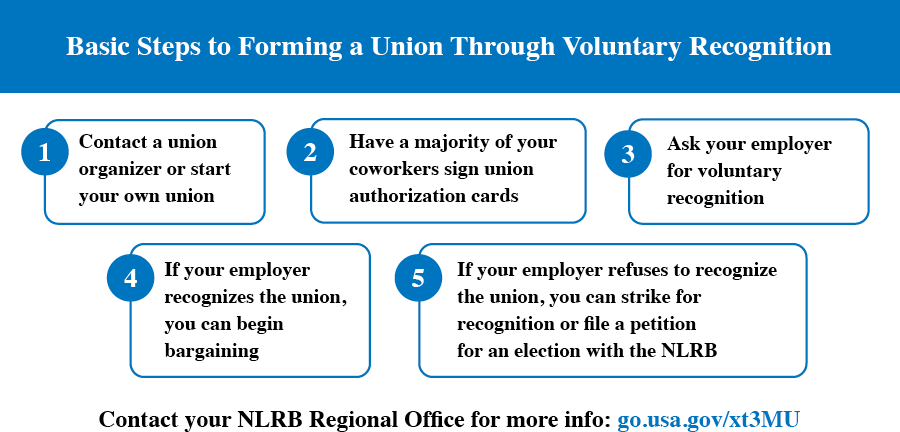
\includegraphics[width=\imageWidth]{images/DOL}
%   \captionsetup{justification=centering, singlelinecheck=false, margin=2cm}
%   \caption[Forming a Union]{The steps for forming a union or joining an existing union. (Source: US Department of Labor.)}
%   \label{fig:DOL}
% \end{figure}

\begin{figure}[ht]
  \centering
  \includegraphics[width=\imageWidth]{images/organizing_paths}
  \captionsetup{justification=centering, singlelinecheck=false, margin=2cm}
  \caption[Union Organizing Paths]{The industrial mode of organizing (left) and the construction mode of organizing (right). Construction unions may follow either path, but other unions may not voluntarily negotiate the way that construction unions can.}
  \label{fig:organizing_paths}
\end{figure}

\begin{figure}[ht]
  \centering
  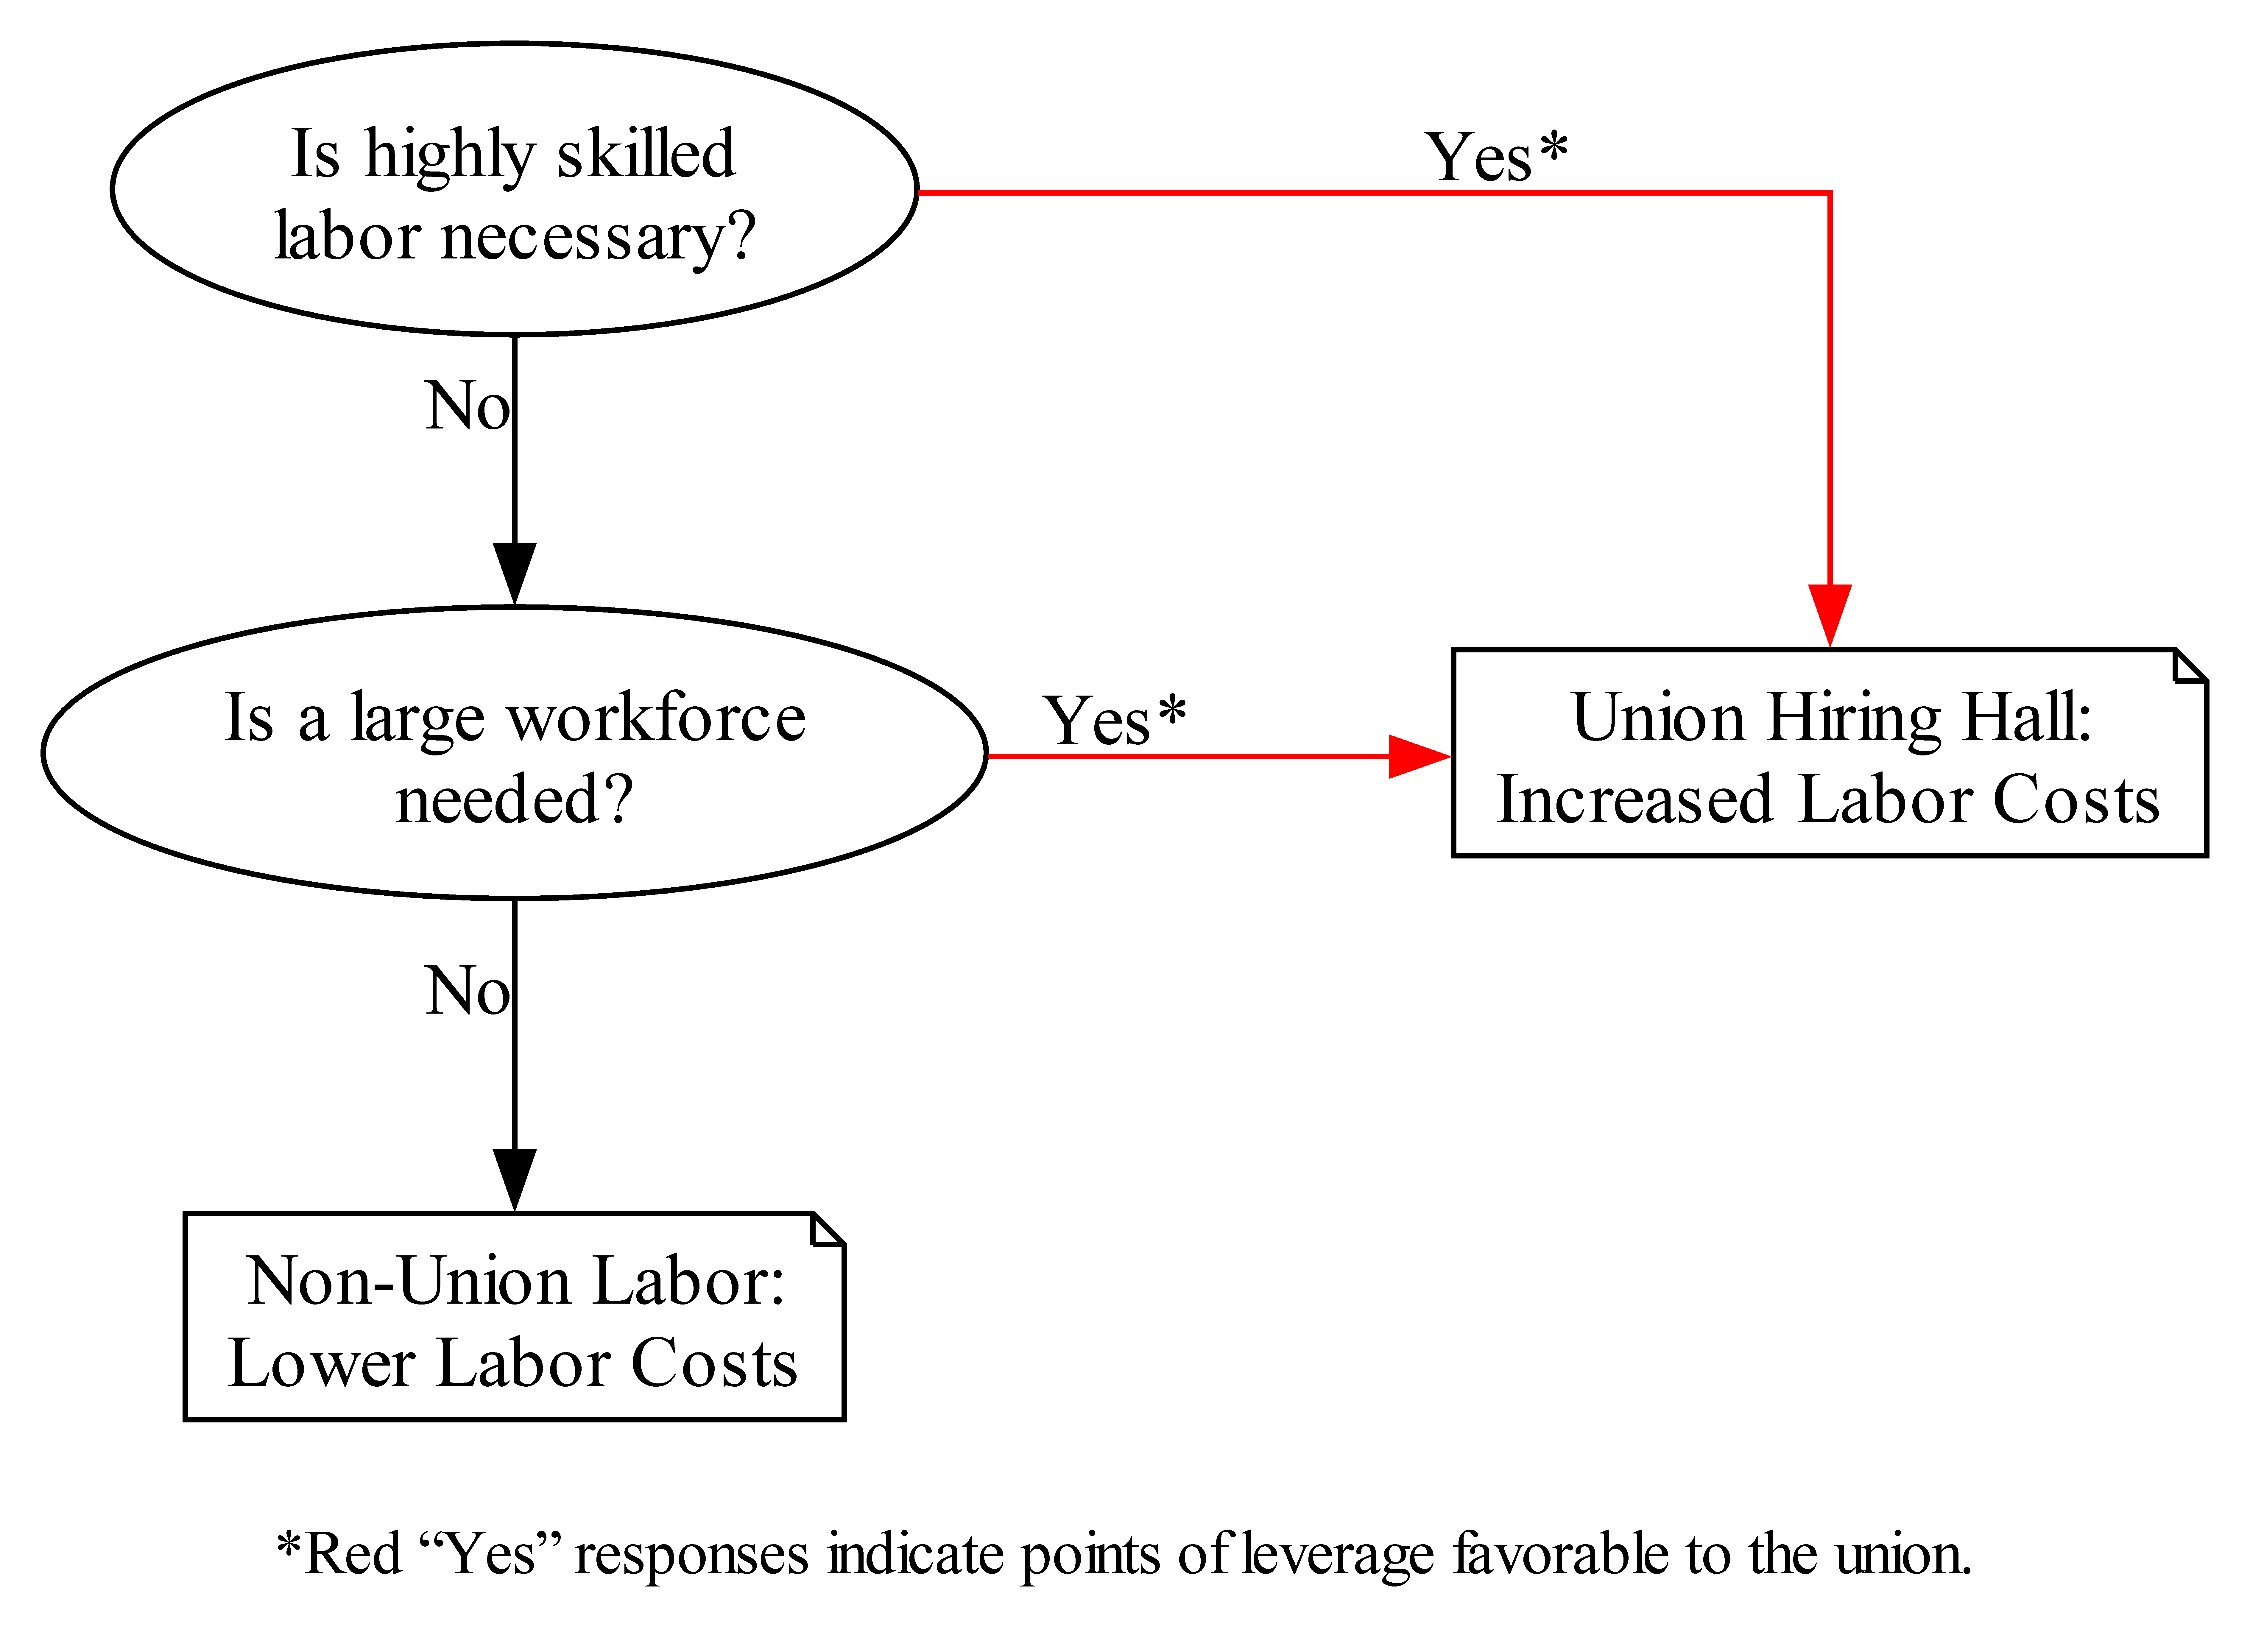
\includegraphics[width=\imageWidth]{images/union_power_red}
  \captionsetup{justification=centering, singlelinecheck=false, margin=2cm} 
  \caption[Union Leverage and Power]{Since negotiations between construction unions and employers are voluntary, construction unions typically have more leverage where the employer requires a more skilled workforce or where the job is large and requires many employees.}
  \label{fig:union_power_red}
\end{figure}

\begin{figure}[!ht]
  \centering
  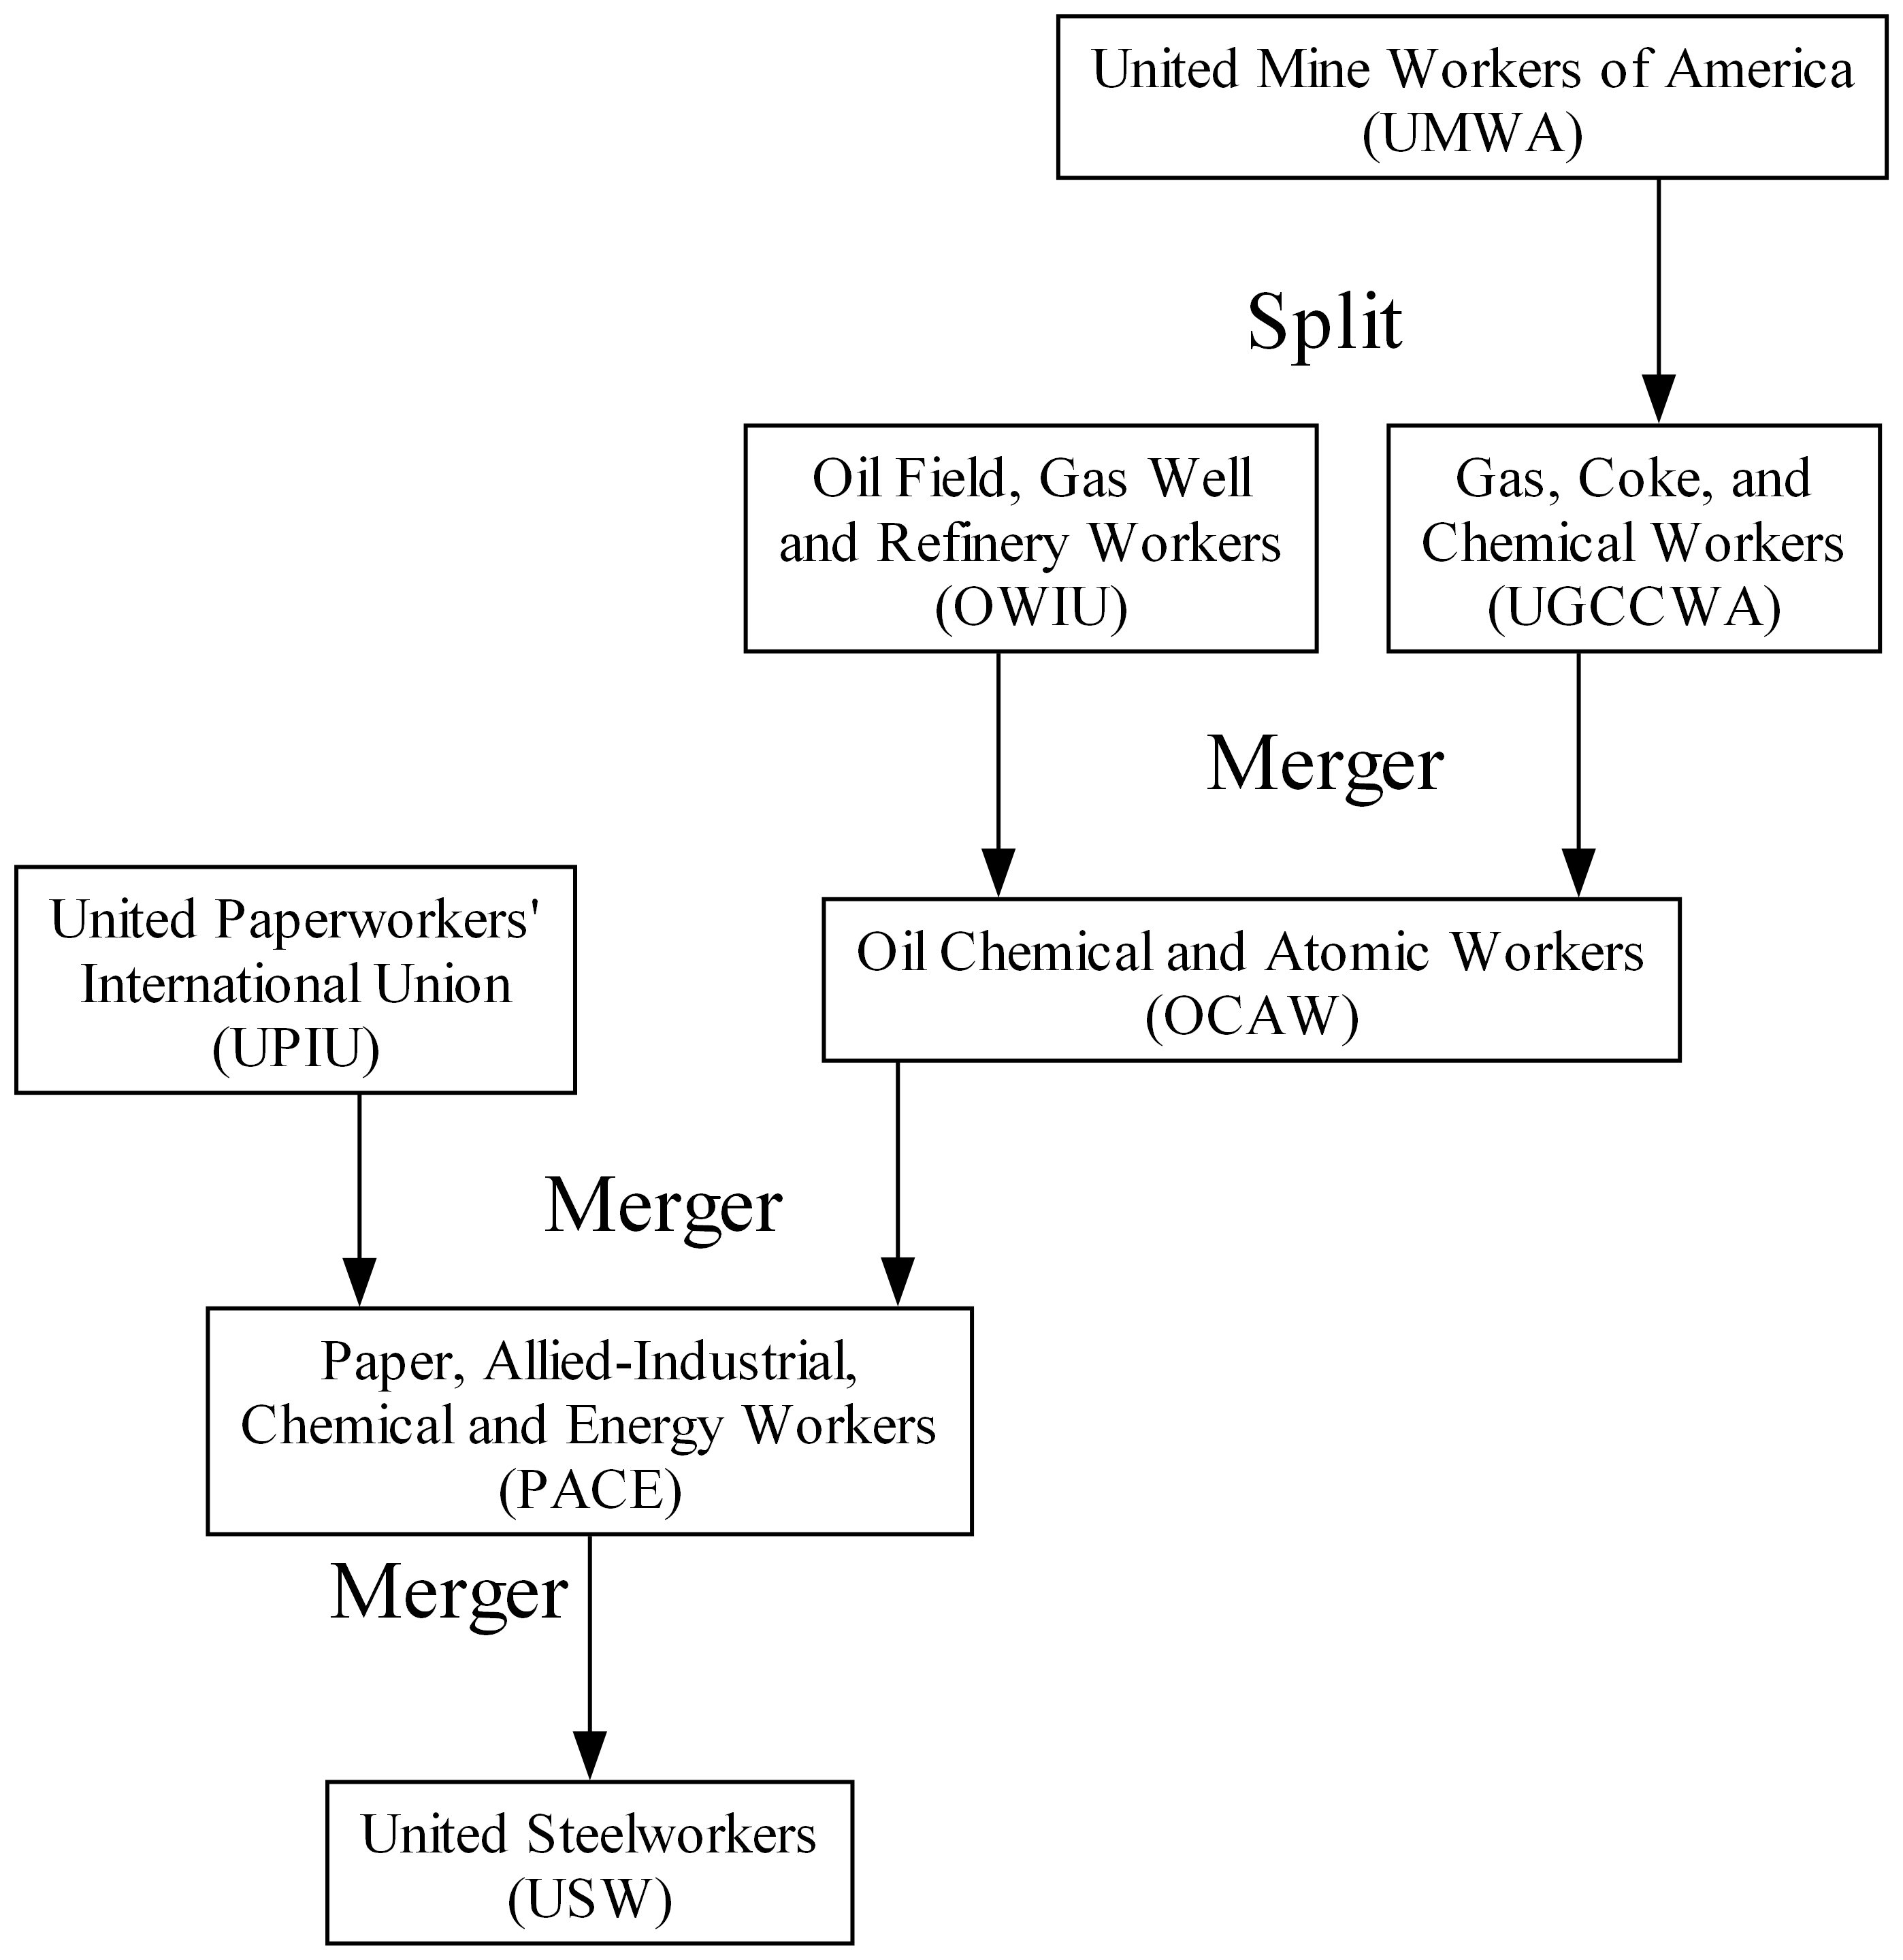
\includegraphics[width=\imageWidth]{images/ocaw}
  \captionsetup{justification=centering, singlelinecheck=false, margin=2cm} 
  \caption[Oil Chemical and Atomic Workers Mergers]{\acrfull{ocaw} was the product of a merger between the \acrshort{owiu} and \acrfull{ugccwa}. It merged with the \acrfull{upiu} in 1999 to form \acrshort{pace}. The \acrshort{ocaw} is now part of the United Steelworkers (\acrshort{usw})}
  \label{fig:ocaw}
\end{figure}


% Uncomment to use end notes instead of footnotes.
%\theendnotes

%%%%%%%%%%%%%%%
%%%% Bibliography %%%%
%%%%%%%%%%%%%%%

% Start on a new page
\clearpage
%\titleformat{\section}{\fontsize{12}{14}\bfseries\centering}{\thesection}{0.5em}{}
\titleformat{\section}[block]
	{\normalfont\fontsize{12}{14}\selectfont\bfseries\centering}
	{\thesection.}
	{0.5em}
	{\MakeUppercase}
	
% Line spacing
\setstretch{1.25}
\sloppy
\printbibliography[heading=bibintoc]% , title=REFERENCES]

\clearpage

% List of acronyms
\addcontentsline{toc}{section}{Acronyms}
%\setglossarystyle{listgroup}
\setlength\glsdescwidth{0.8\linewidth}
\printglossary[type=\acronymtype, title=Acronyms, style=long]
\clearpage

%\paperwidth=\pdfpagewidth
%\paperheight=6.5in
%\pdfpageheight=8.5in % keep at 8.5 in
%\pdfpagewidth=11in % keep this at 11 in
%\headwidth=8.5in % keep this at 11 in

%\fancypagestyle{lscape}{% 
%\fancyhf{} % clear all header and footer fields 
%\fancyhead[L]{%
%\begin{textblock}{1}(1,15){\rotatebox{90}{test}}\end{textblock}
%\begin{textblock}{1}(13,15){\rotatebox{90}{\thepage}}\end{textblock}
%}}


%\newpage
%\paperwidth=\pdfpageheight
%\paperheight=\pdfpagewidth
%\pdfpageheight=\paperheight
%\pdfpagewidth=\paperwidth
%\headwidth=\textwidth

\end{document}
